%!TEX root = ../icip_jseo.tex
% -*- root: ../icip_jseo.tex -*-

\section{Introduction}
\label{sec:intro}

Image matching is a fundamental problem in a variety of computer vision applications, including object recognition\cite{nister_scalable_2006}, panorama stitching\cite{brown_recognising_2003}, and augmented reality\cite{wagner_multiple_2009}. To accomplish image matching, keypoint-based local matching is widely used, since it can provide relatively high matching quality against severe occlusion and do not require segmentation for regions of interest. Also, recent work has concentrated on making invariant to image transformation with low computing power\cite{carrera_robust_2007,mikolajczyk_performance_2005}.

% To enhance the image matching quality in various environments, many related techniques have been proposed, such as keypoint-based local matching, histogram-based global matching\cite{le_improving_2013}, color-based matching\cite{mehtre_color_1995}, and template-based matching\cite{korman_fast-match:_2013}, etc. Among them, keypoint detection and matching has created great interest 

The overall flowchart of keypoint matching and recognition is shown in Fig. \ref{fig:on_offline_process}. This procedure can be divided into two main phases: offline learning (or training) and online testing procedure. Offline learning is a prerequisite to online matching process. In offline learning phase, a set of reference images to be recognized is analyzed and stored a set of descriptors in a database. In online testing phase, a newly captured image is analyzed and compared with the reference images in the database to find a nearest reference image. 
% In each phase, common procedures for matching are keypoint detection, description, and matching. To analyze training images, at first, keypoints are detected from the images. Then, from those keypoints, local textures are analyzed and described. In this procedure, to provide robustness against rotation, scale, perspective transform, descriptors are constructed. Then, to be used in online phase, efficient matching structures, as databases, are constructed, such as partitioning trees\cite{arya_optimal_1998,beis_shape_1997}, hashing\cite{salakhutdinov_semantic_2009,lv_multi-probe_2007}. In the online matching phase, the database is used to find the most similar corresponding keypoints pair with a given query image. To find the most similar keypoint pairs, with given a query image, keypoints are detected, detected keypoints are described about local texture, and compared with the preconstructed database.

\begin{figure}[hb!]
\centering
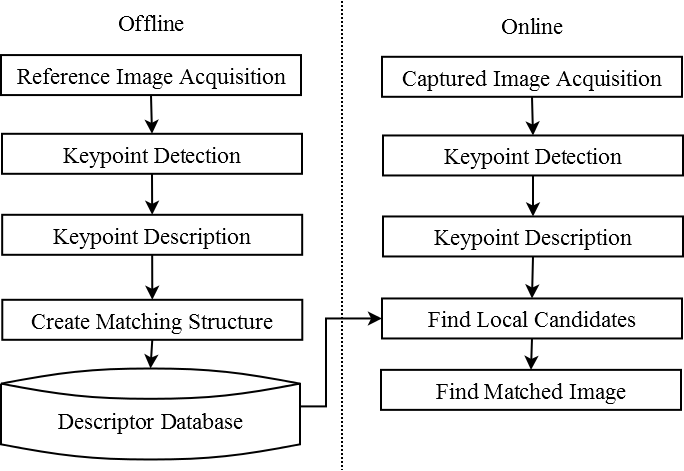
\includegraphics[width=1.0\columnwidth]{1_introduction/process}
\caption{Overall process of conventional keypoint-based matching}
\label{fig:on_offline_process}
\end{figure}

Conventional keypoint matching methods stores almost every keypoints which are detected by keypoint detection process. Keypoint detection processes are designed to extract repeatable keypoints and robust against arbitrary image transformation. Then, detected keypoints are independent to the follow matching procedures, and do not reflect quality of descriptors. Therefore, as seen Fig. \ref{fig:example_of_bad_features}, some keypoints are not distinguishable, and they tend to cause inter-keypoint confusion and miss matching. Also, those detected keypoints are stored in database and are compared with keypoints in query images in every frame while matching. Then, it decreases the speed of matching. To overcome these problem, in offline learning procedure, detected keypoints are evaluated with respect to proposed matching quality criteria and filtered by the goodness score. With this filtering method, only a small subset of keypoints is stored in the database. Accordingly, it provides more improved matching performance with faster matching speed.

\begin{figure}[ht!]
\centering
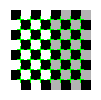
\includegraphics[width=0.5\columnwidth]{1_introduction/checkerboard}
\caption{Example of high repeatable but poor distinguishable keypoints. Conventional keypoint matching systems do not consider the discriminability of keypoints, so these keypoints usually stored and negatively affected matching.}
\label{fig:example_of_bad_features}
\end{figure}

Especially, mobile devices still have insufficient computing power and limited memory compared to desktop, so there is an urgent need of effective processing methods for image matching. However, conventional keypoint matching approaches stored redundant keypoints into database, and these redundant keypoints may are compared in every frame. So, matching speed will be decreased and this causes problem in the mobile computing devices. On the other hand, the proposed method removes redundant keypoints in the database, it reduces the number of comparisons while matching and increase matching speed even in the mobile computing environment.

This paper is structured as follows: In Chapter 2, we discuss literature on light-weight keypoint-matching algorithms. Chapter 3 describes the proposed keypoint score function. In Chapter 4, we executed experiments to prove the proposed keypoint filtering method in various algorithms and compared over several evaluation metrics. Finally, Chapter 5 presents the conclusion.
